\usepackage[authoryear,round]{natbib}
\usepackage{multirow}

\newcommand{\sheetnum}{%
	09
}
%\setcounter{section}{\sheetnum-3}
\newcommand{\tutorialtitle}{%
    Self-Organizing Maps
}
\newcommand{\tutorialtitleshort}{%
	SOM
}
% for slides
\subtitle{\sheetnum \tutorialtitle}

\maxdeadcycles=1000 % Workaround for ! Output loop---100 consecutive dead cycles because of too many figures

% The following use of algroithms is recommended for the notes:
%
%\begin{figure}[!t]
%\removelatexerror
%\begin{algorithm}[H]
    % your algo here
    %\label{alg:algolabel}
    %\caption{algocaption}
%\end{algorithm}
%\end{figure}
%\begin{algorithm}
% Below is the definition for the command \removelatexerror:
\makeatletter
\newcommand{\removelatexerror}{\let\@latex@error\@gobble}
\makeatother

\begin{document} %%%%%%%%%%%%%%%%%%%%%%%%%%%%%%%%%%%%%%%%%%%%%%%%%%%%%%%

\sheet{\sheetnum}{\tutorialtitleshort}

\ttopic{\tutorialtitle}

\begin{frame}
\titlepage
\end{frame}

%\setcounter{tocdepth}{2}
%\begin{frame}
%\mode<presentation>{
%\tableofcontents[subsubsectionstyle=show/show/show/hide]
%}
%\mode<article>{
%\tableofcontents
%}
%\end{frame}
\begin{frame}
\mode<presentation>{
\tableofcontents[hideallsubsections]
}
\mode<article>{
\tableofcontents
}
\end{frame}

\newpage

% The variable mycolumnleft is set in the minotes class
% The column settings are ignored by the slides
\columnratio{\mycolumnleft,1-\mycolumnleft}
\begin{paracol}{2}
%\setlength{\columnseprule}{0.1pt}
%\setlength{\columnsep}{5em}

\begin{rightcolumn}

\mode<all>
\section{Remarks to Clustering}

\mode<presentation>{
\begin{frame} 
    \begin{center} \huge
        \secname
    \end{center}
    \begin{center}
		No relationships between clusters
    \end{center}
\end{frame}
}

\subsection{K-means Sinusoid example}

\begin{frame}{\subsecname}

Consider the following 2-D data and applying K-means with $M=7$ prototypes.

\begin{minipage}{0.45\textwidth}
\begin{center}
	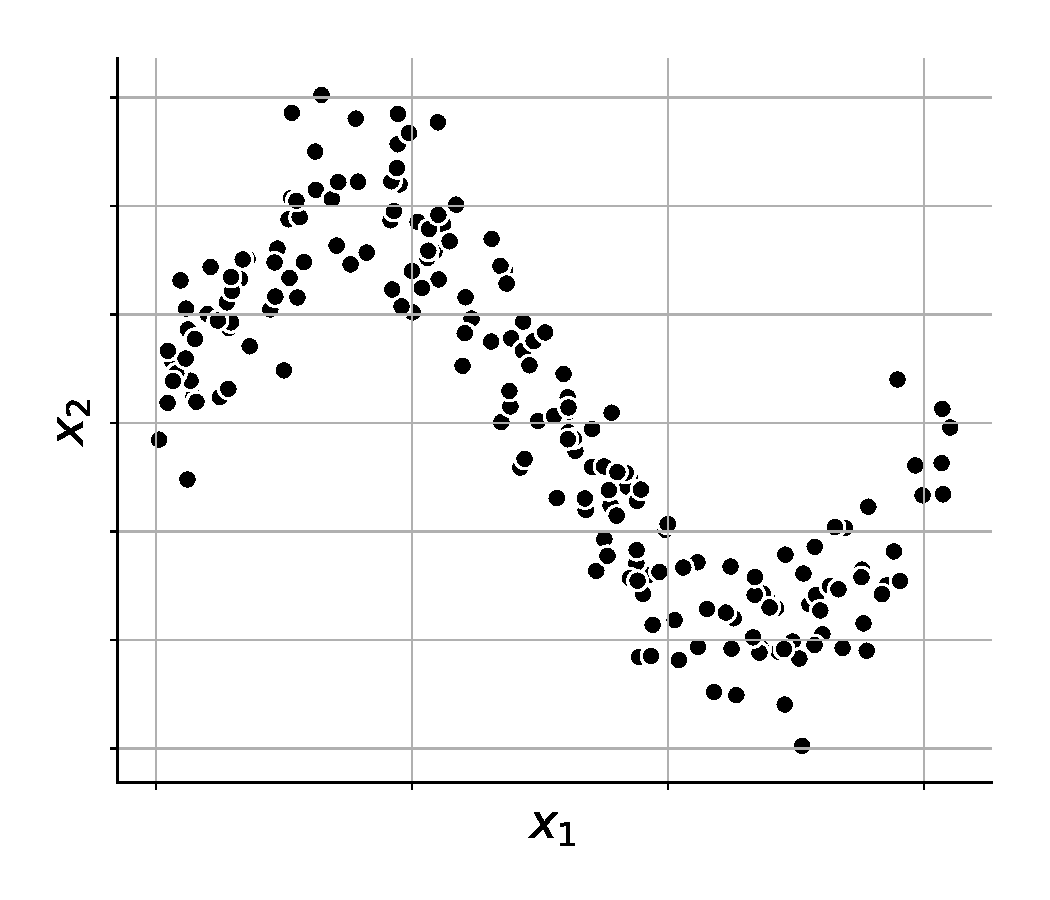
\includegraphics[width=0.8\textwidth]{img/sin_data}
	\notesonly{\captionof{figure}{2D points describing a sinusoid.}}
\end{center}
\end{minipage}
\begin{minipage}{0.45\textwidth}
\begin{center}
	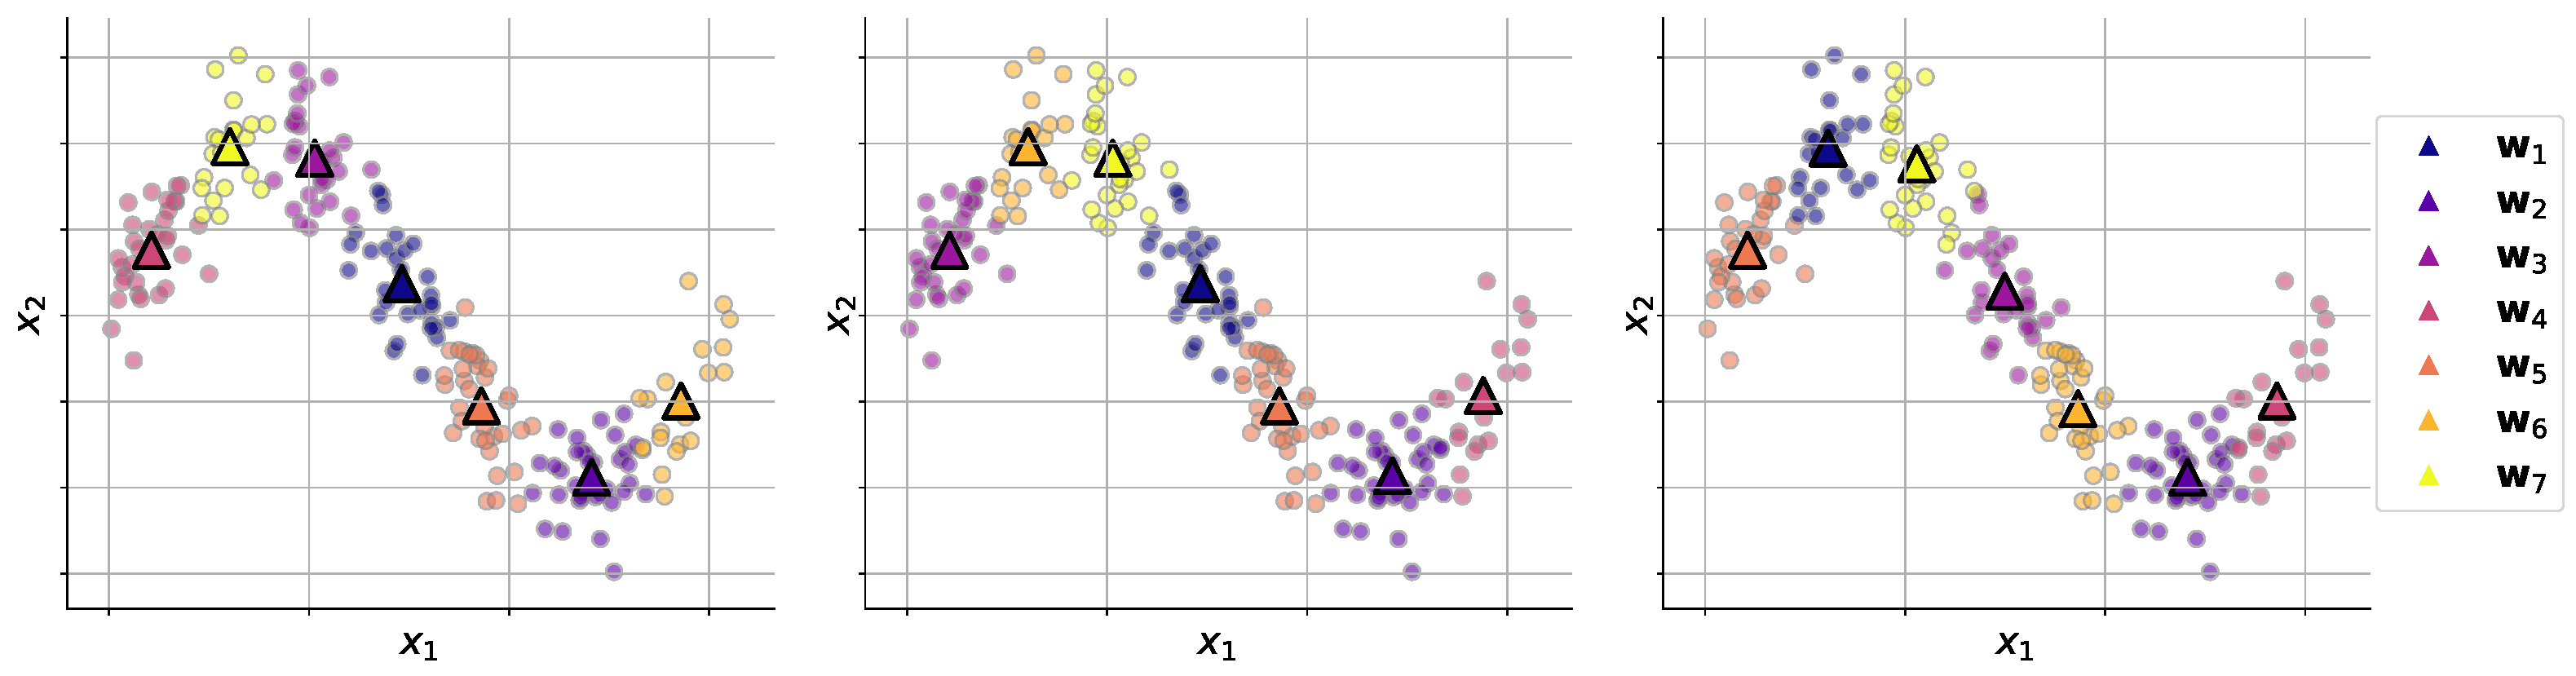
\includegraphics[trim=950 0 0 0,clip, width=0.9\textwidth]{img/sin_clustering}
	\notesonly{\captionof{figure}{A clustering solution with 7 prototypes.}}
\end{center}
\end{minipage}

\end{frame}

\begin{frame}{Multiple runs of K-means on the data}

\begin{center}
	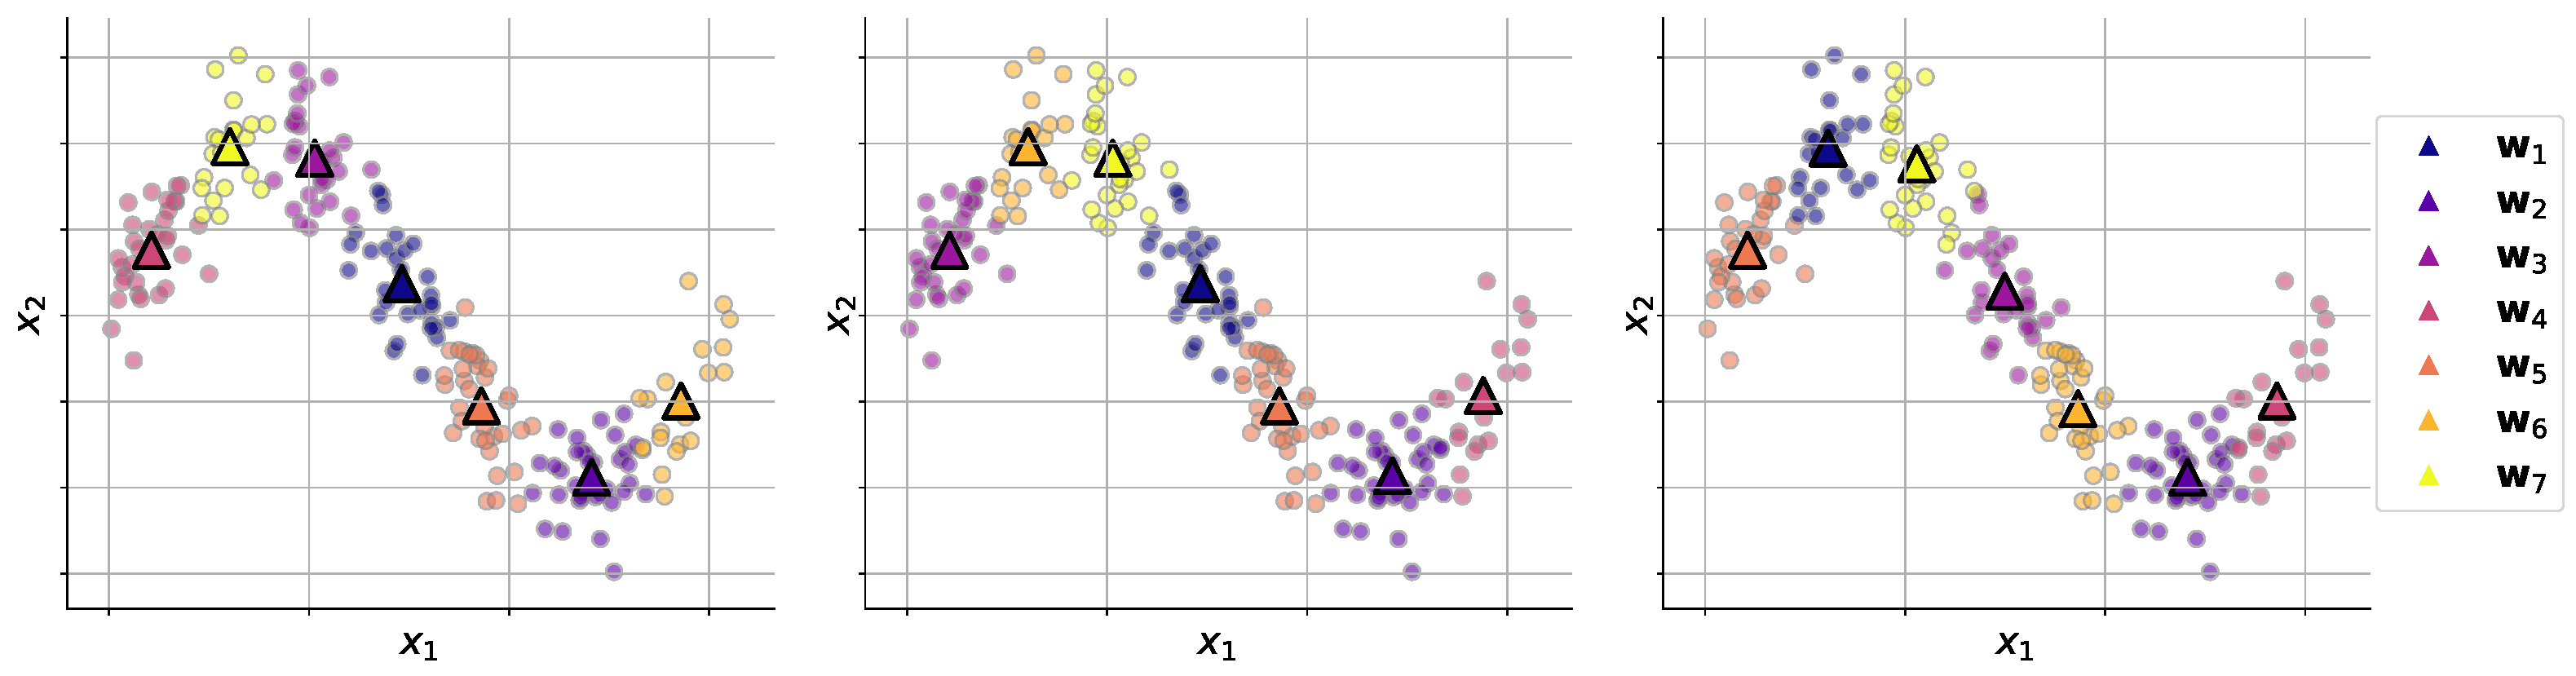
\includegraphics[width=0.95\textwidth]{img/sin_clustering}
	\captionof{figure}{Equivalent clustering solutions with 7 prototypes.}
\end{center}

\begin{itemize}
\item The clustering solutions are equivalent in that they are permutations of one another.
\item There is no ``order'' in the numbering of the cluster indices. The numbers don't reflect any topology about the clusters.
\end{itemize}

\end{frame}

\begin{frame}{Reflect topology by sorting the cluster indices}

Renumber the cluster indices by sorting the prototypes according to position along the horizonal axis.

\begin{center}
	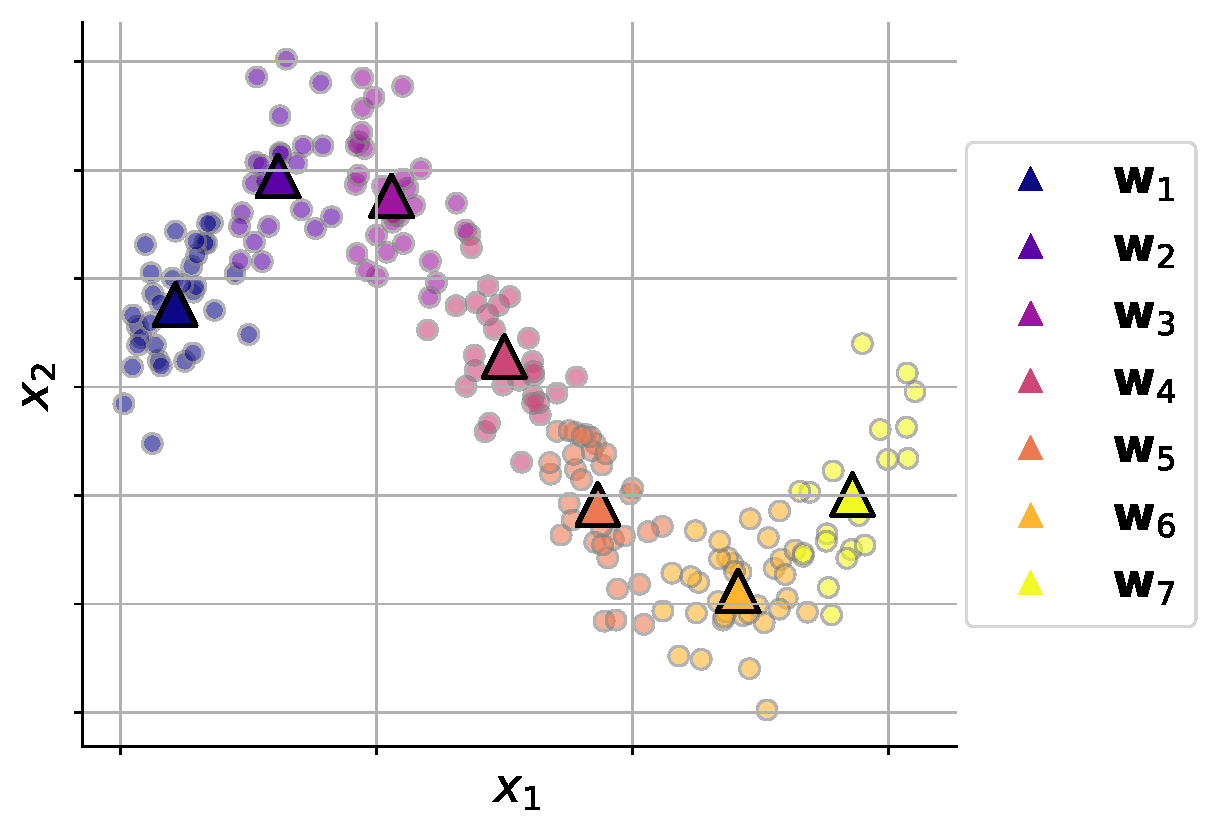
\includegraphics[width=0.5\textwidth]{img/sin_clustering_sorted}
	\notesonly{\captionof{figure}{Equivalent clustering solution with 7 prototypes that reflects some topology in the data.}}
\end{center}

$\vec w_{q}$ and $\vec w_{q+1}$ are neighbors in input space.

\end{frame}

\subsection{Motivation for clustering that preserves neighborhood}

\begin{frame}{\subsecname}

Recap from last time\\

\question{What does clustering give us?}
 
\begin{itemize}
\item[-] Discrete low-dimensional representation of data points.
\begin{equation}
\text{point}~\vec x \in \R^N \quad \longrightarrow \quad~\text{cluster index}~q \in \N
\end{equation} 
\item We will be able to describe the entire dataset by the partitions we've found that separate the clusters.
\item We'll draw relations between simple clustering and other algorithms (\textbf{embedding} algorithms, density estimation)
\end{itemize}

\end{frame}

\begin{frame}

\begin{block}{Embedding}

A low-dimensional representation of the data that is neighborhood preserving,
\begin{itemize}
\item[i.e.] account for local structure,
\item[e.g.] two points close in $N$-dim input space should remain close in the low-dimensional embedding space.
\end{itemize}

\end{block}

\end{frame}

\begin{frame}{A step towards manifold learning}

\begin{block}{The manifold: a handwavy explanation}

The space in which data resides that is possibly much lower than the $N$-dimensional space we observe it in.
It is a space in which we draw any insights from the data just as we try to do from the $N$-dim. observations (e.g. clustering, classifcation,...)

\end{block}

\pause

\begin{center}
	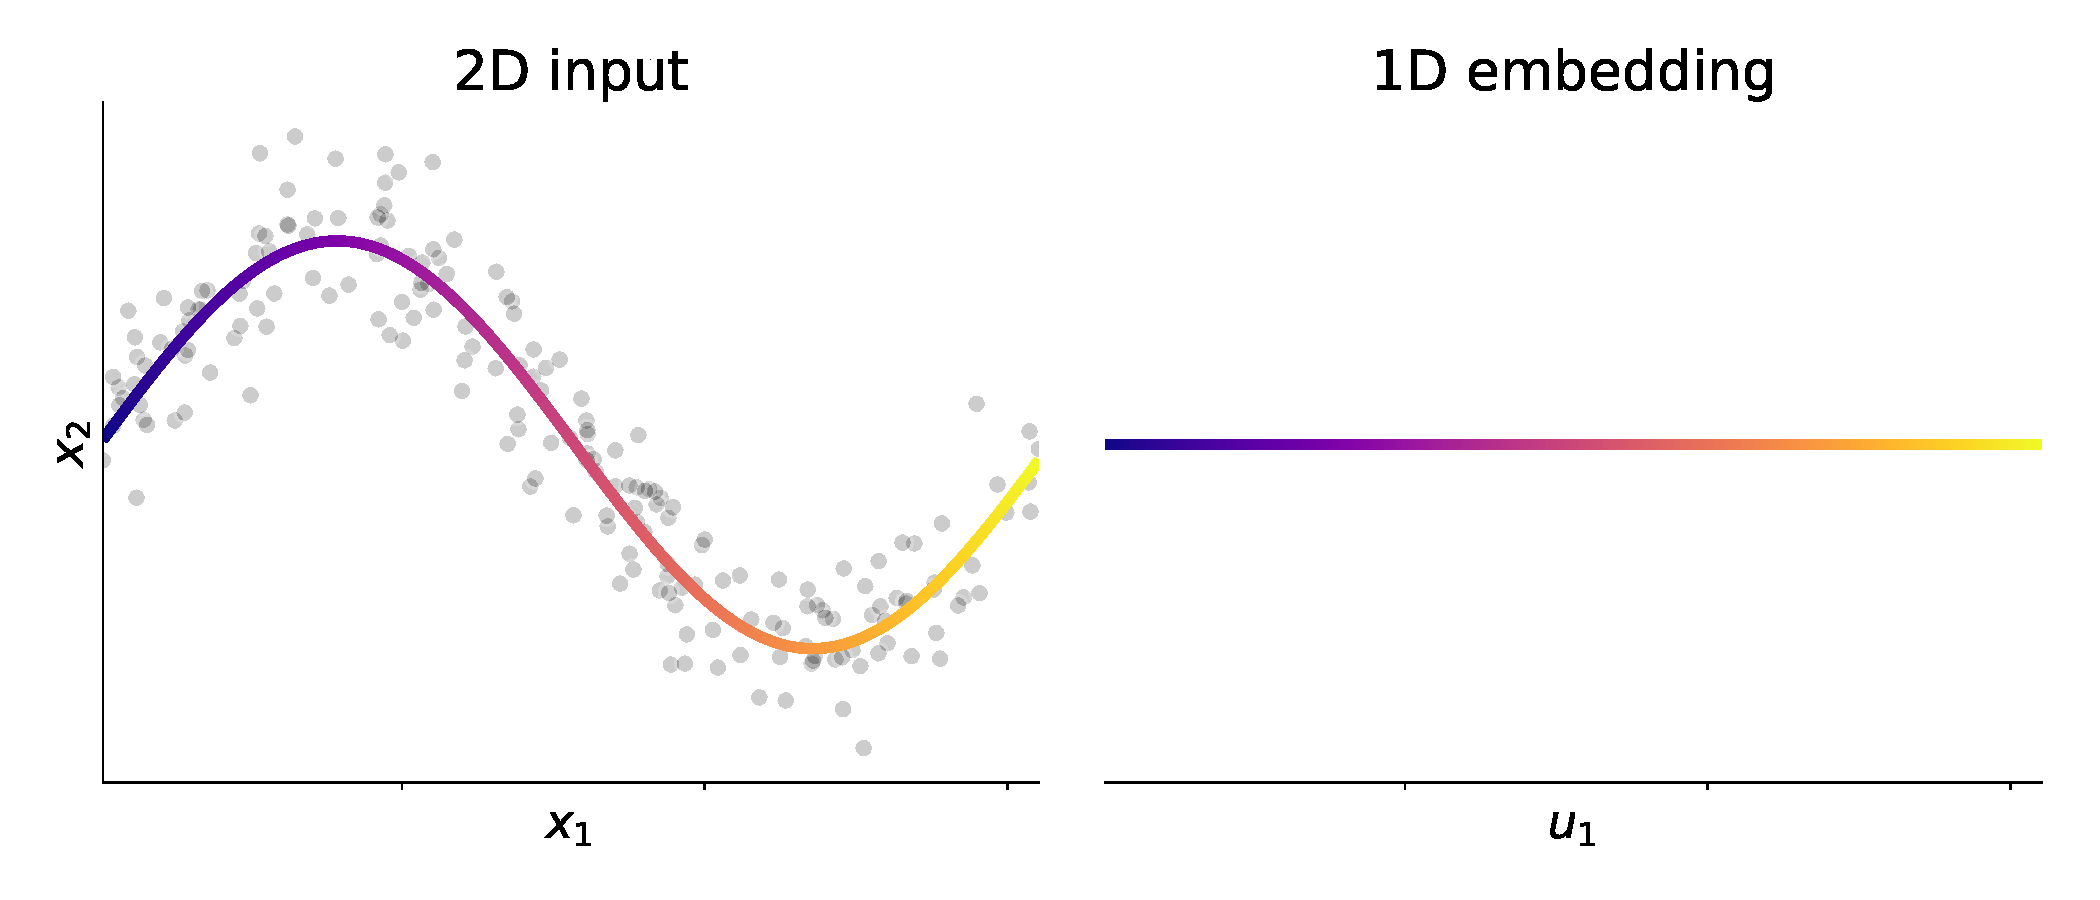
\includegraphics[width=0.8\textwidth]{img/sin_manifold}
	\captionof{figure}{A 1D embedding of the 2D sinusoidal curve}
\end{center}

\end{frame}

\begin{frame}{An ant's perspective}
\notesonly{Looking at data from the perspective of an \emph{ant}.}

\begin{center}
	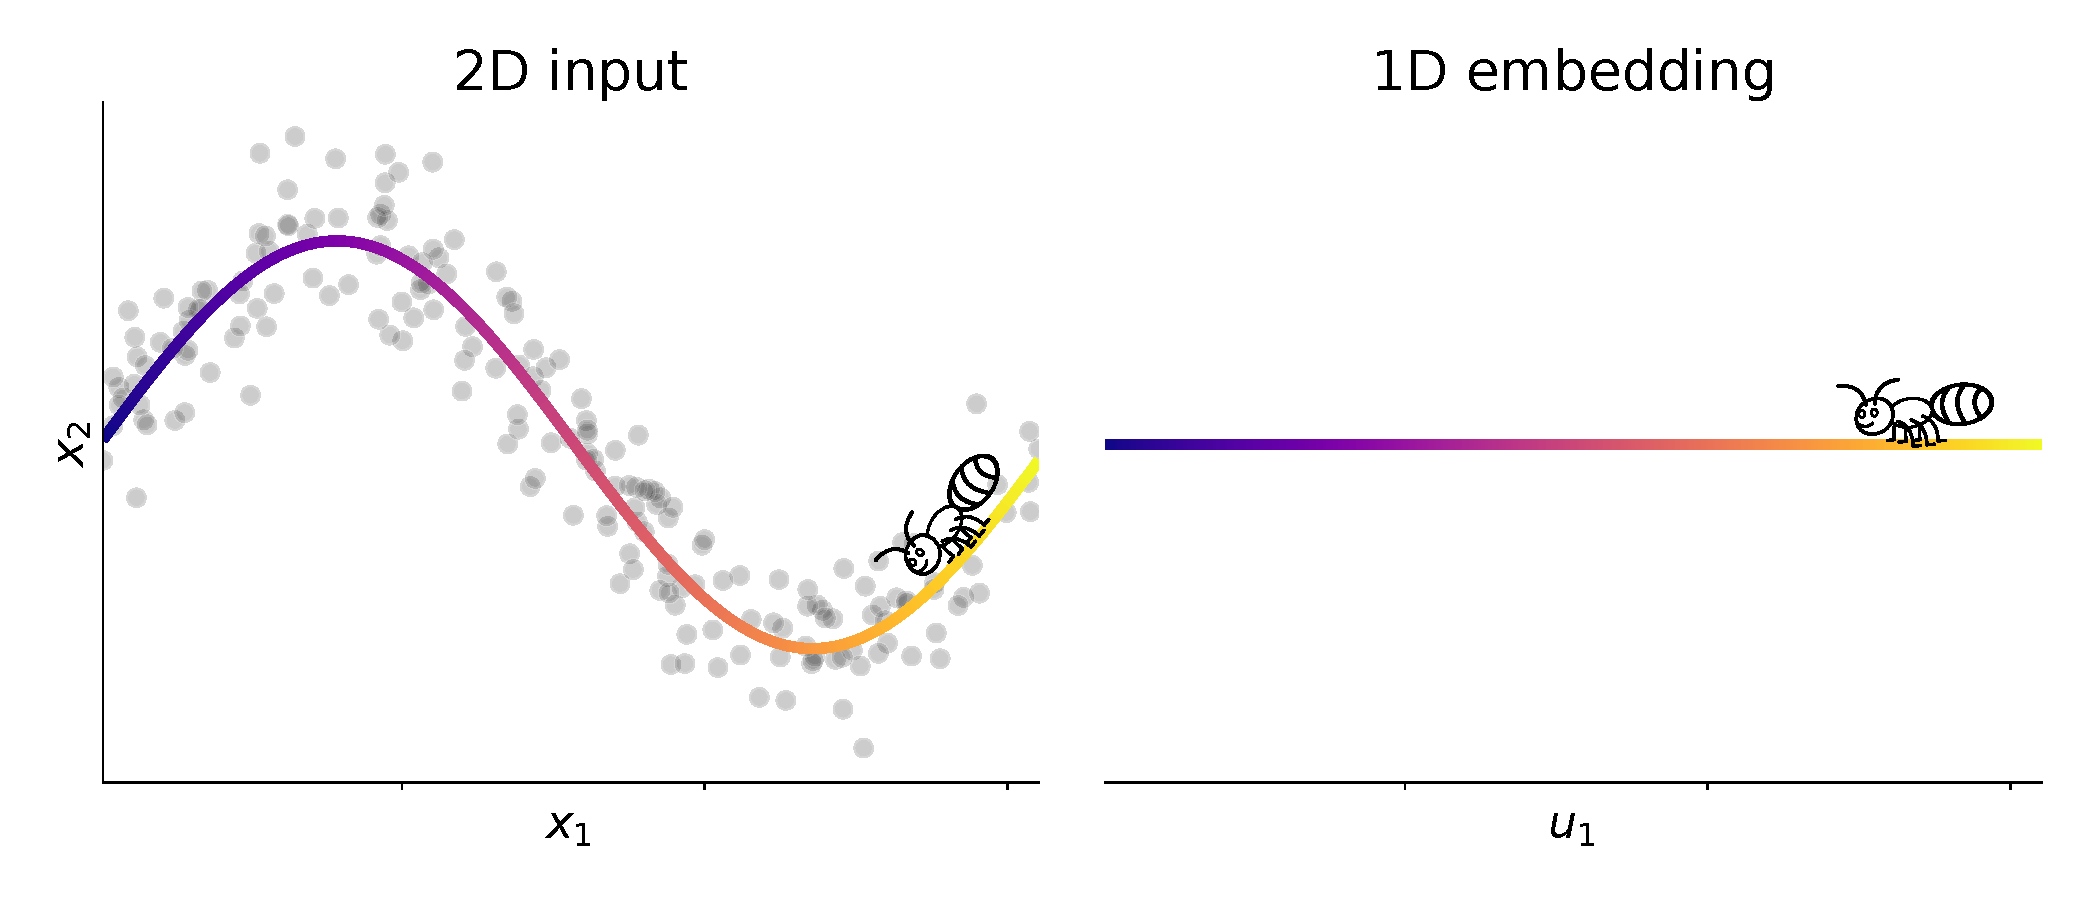
\includegraphics[width=0.9\textwidth]{img/sin_manifold_ant}
	\captionof{figure}{To the little ant, the sinusoid is just a 1D line. No turns, no elevation.}
\end{center}

\end{frame}

\begin{frame}

\slidesonly{
\begin{center}
	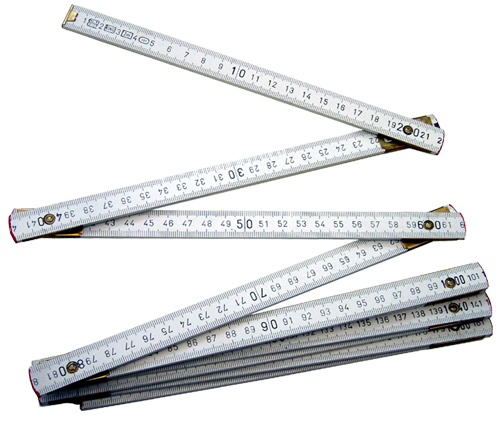
\includegraphics[width=0.3\textwidth]{img/Metre_pliant_500px}
	\captionof{figure}{Zollstock - Carpenter's rule}
\end{center}
}

\end{frame}

\begin{frame}{A discrete mapping}

\begin{center}
	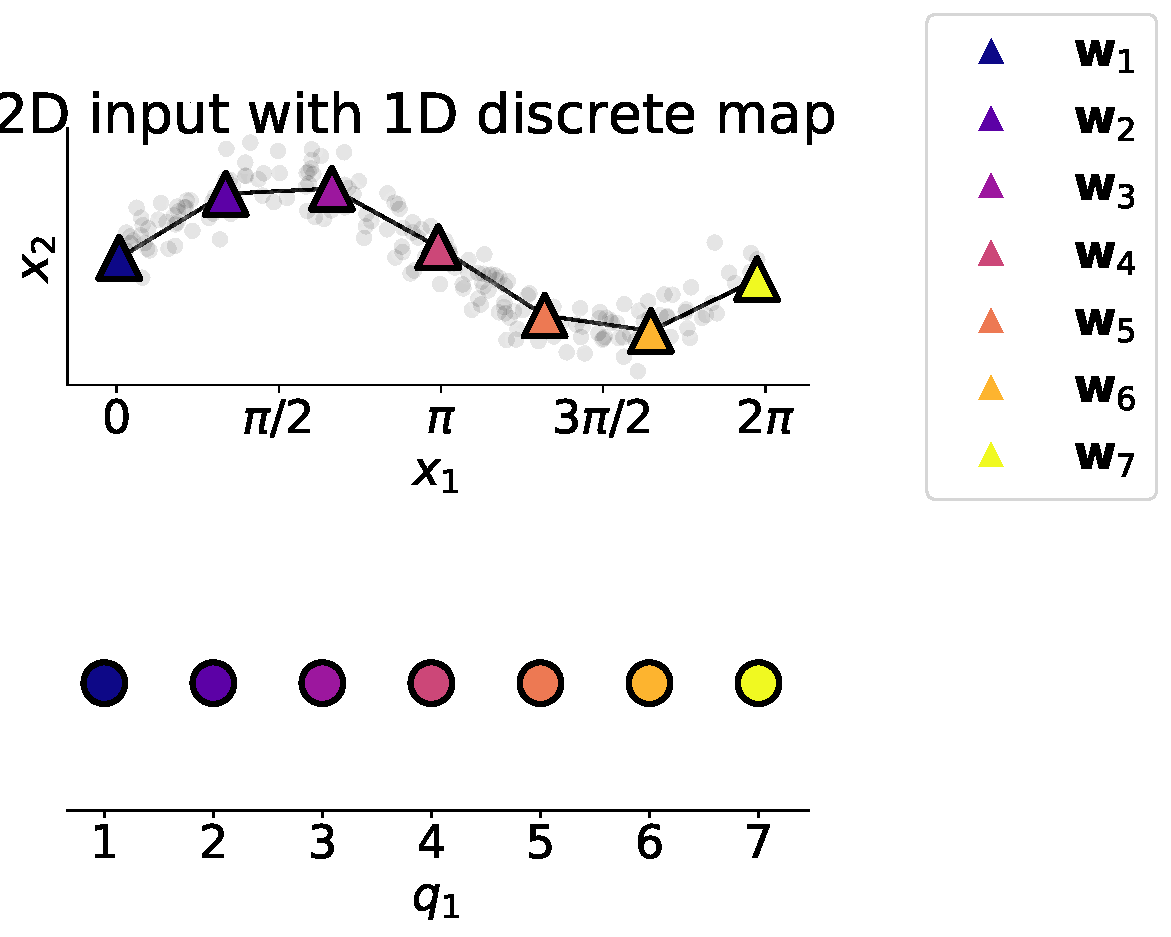
\includegraphics[width=0.6\textwidth]{img/sin_manifold_map}
	\captionof{figure}{2D input with a discrete mapping (e.g. SOM)}
\end{center}

\end{frame}

\mode*

\clearpage

\mode<all>
\section{Self-Organizing Maps (SOM)}

\mode<presentation>{
\begin{frame} 
    \begin{center} \huge
        \secname
    \end{center}
    \begin{center}
		Neighborhood-preserving clustering to explain the data
    \end{center}
\end{frame}
}

\subsection{The model class}

\begin{frame}{\subsecname:~The components SOM model}

\only<1-2>{
\svspace{-3mm}
\begin{center}
	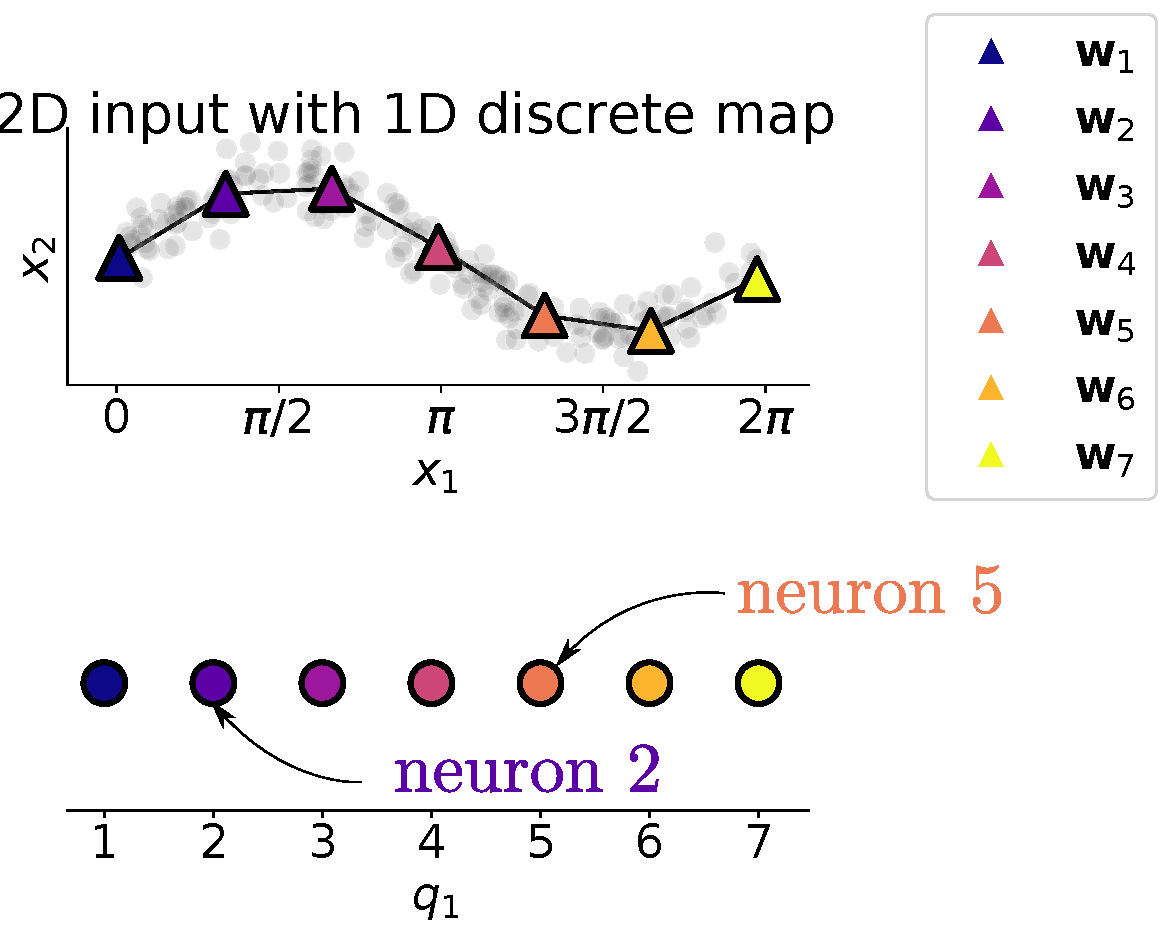
\includegraphics[width=0.5\textwidth]{img/sin_manifold_map_annot}
	\notesonly{\captionof{figure}{The 1D SOM model}}
\end{center}
}
\only<3>{
\begin{center}
\begin{minipage}{0.29\textwidth}
	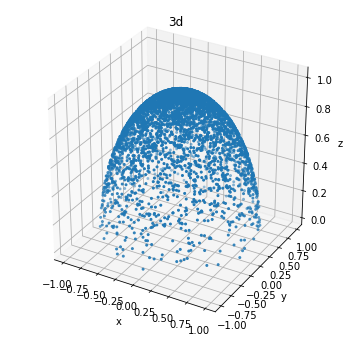
\includegraphics[width=0.9\textwidth]{img/3-a}
	\notesonly{\captionof{figure}{Bowl-shaped data in 3 dimensions}}
\end{minipage}
\begin{minipage}{0.29\textwidth}
	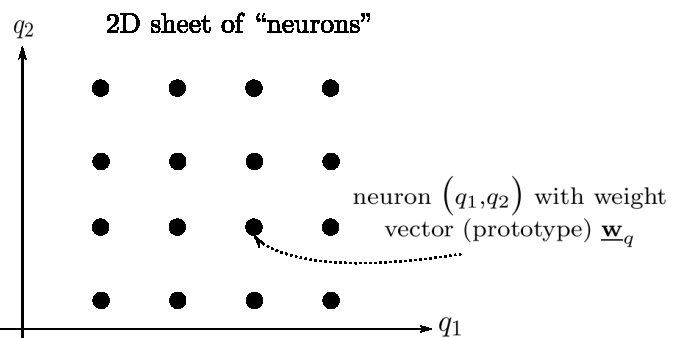
\includegraphics[width=0.99\textwidth]{img/section4_fig8}
	\notesonly{\captionof{figure}{a 2D map of neurons}}
\end{minipage}
\begin{minipage}{0.29\textwidth}
	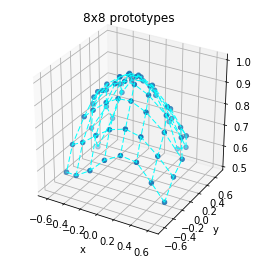
\includegraphics[width=0.9\textwidth]{img/3-b}
	\notesonly{\captionof{figure}{Prototypes fitted to the data.}}
\end{minipage}
\end{center}
}

\begin{itemize}
\only<1>{
\item The neurons form a map in a lower dimensional space.
\item The map space is discrete with coordinates $\vec q$ to describe the position of every neuron in the map (lattice)
\item Each neuron is associated with a prototype $\vec w_{\vec q}$ that lives in $N$-dim input space.
}
\only<2>{

\newpage

\item In the case of a 1D map:
\begin{itemize}
\item The neurons form a chain in map space.
\item Each neuron is associated with single coordinate $q_1$ to describe its position in the chain.
\item The dimensionality of a neuron's prototype $\vec w_{q_1}$ lives in $N$-dim space (i.e. that of the input)
\end{itemize}
}
\only<3->{
\item In the case of a 2D map:
\begin{itemize}
\item The neurons form a grid (lattice) in map space.
\item Each neuron is associated with coordinates $\vec q = (q_1, q_2)^\top$ to describe its position in the grid.
\item The dimensionality of a neuron's prototype $\vec w_{\vec q}$ lives in $N$-dim space (i.e. that of the input)
\end{itemize}
}
\end{itemize}

\end{frame}

\begin{frame}%{\subsecname}

\question{What is the role of the coordinates $\vec q$ of a neuron?}

\pause

\begin{itemize}
\item It describes the neuron's position in the map. It gives us access to the neighbors of this neuron in the map.
\item This enables organizing the neurons such that the response of two neighboring neurons is more similar than that of two neurons that are far away from one another (cooperation)
\end{itemize}

\end{frame}

\begin{frame}%{\subsecname}

\question{What is the role of the prototypes $\vec w_{\vec q}$ of a neuron?}

\pause

\begin{itemize}
\item It connects the neuron to the data.
\item Enables the assignment of a sample $\vec x^{(\alpha)}$ with $\vec x \in \R^N$ and $\alpha = 1,\ldots,p$ to a neuron.\\
This is essentially clustering, but now with the possibility of a multidimensional cluster $\vec q$: \\
\begin{equation}
	m_{\vec{q}}^{(\alpha)} = \left\{ \begin{array}{ll}
		1, & \text{if } \vec q = \underset{\vec r}{\argmin} \big| \vec{x}^{(\alpha)}
			-\vec{w}_{\vec r} \big| \\\\
		0, & \text{otherwise}
	\end{array} \right.
\end{equation}
The clustering aspect can be viewed as a \emph{competition} between the neurons.
\item All prototypes collectively provide an explanation for the data. i.e. ``a 2D sheet or 1D chain that covers the space in $N$-dim space that is occupied by the data''
\end{itemize}

\end{frame}

%\subsection{Comparing SOM to clustering}

%\begin{frame}{\subsecname}

%\begin{itemize}
%\item In common:
%\begin{itemize}
%\item Protoypes live in space of the input
%\end{itemize}
%\item Differences:
%\begin{itemize}
%\item 
%\end{itemize}
%\end{itemize}

%\end{frame}

\mode*

\clearpage

\mode<all>
\section{The SOM learning algorithm}

\mode<presentation>{
\begin{frame} 
    \begin{center} \huge
        \secname
    \end{center}
    \begin{center}
		Compete, Cooperate and Adapt\\
		Learn to ``cover''/``explain'' the data
    \end{center}
\end{frame}
}

% --------------------------------------------------------------------------
\begin{frame}[shrink=1] 
\begin{figure}[!th]
\footnotesize
\removelatexerror
\begin{algorithm}[H]
\DontPrintSemicolon  
\textbf{Initialization:} \;
- choose no. $M$ of partitions (``neurons'') \textcolor{red}{and the topology of the map}\;
- choose annealing schedule for $\varepsilon$ and $\sigma$\;
- initialize $M$ prototypes: $\vec{w}_{\vec q} = 1/p \sum_\alpha \vec{x}^{(\alpha)}+\vec{\eta} $, \hspace{0.3cm}$\vec{\eta}$ small noise vector \;
\Begin(){
  choose a random data point $\vec{x}^{(\alpha)}$ \\
  determine the closest prototype:\[ \vec{p} = \underset{\vec r}{\argmin} \big| \vec{x}^{(\alpha)} - \vec{w}_{\vec r} \big|\] \\
  change all prototypes $\vec{w}_{\vec q}$ according to: $$\Delta \vec{w}_{\vec q} = \varepsilon \cdot h_{\vec{q} \, \vec{p}} \cdot 
  \big( \vec{x}^{(\alpha)} - \vec{w}_{\vec q} \big) \text{\hspace{1cm} for \textcolor{red}{all} \vec{q}}$$ \\
  lower the learning rate $\varepsilon$ and neighborhood width $\sigma$
}
\label{alg:kohonen}
\caption{On-line learning for SOM}
\end{algorithm}
\end{figure}

\end{frame}

\subsection{The neighborhood function}

% --------------------------------------------------------------------------
\begin{frame}[t] \frametitle{\subsecname~$h_{\vec{q} \, \vec{p}}$} 
\begin{equation}
	\Delta \vec{w}_{\vec q} = \varepsilon \cdot h_{\vec{q} \, \vec{p}} \cdot
  \big( \vec{x}^{(\alpha)} - \vec{w}_{\vec q} \big) \text{\hspace{1cm} for \textcolor{red}{all} q}
  \end{equation}
\begin{itemize}
	\item $h_{\vec{q} \, \vec{p}}$ enforces similar learning steps for neighboring neurons
	\item common choice:
	\begin{equation}
		h_{\vec{q} \, \vec{p}} = \exp \bigg\{ - \frac{ (\vec{q}
			- \vec{p} )^2 }{2 \sigma^2} \bigg\}
			\end{equation}
\end{itemize}

\begin{center}
\begin{minipage}{0.4\textwidth}
\begin{center}
	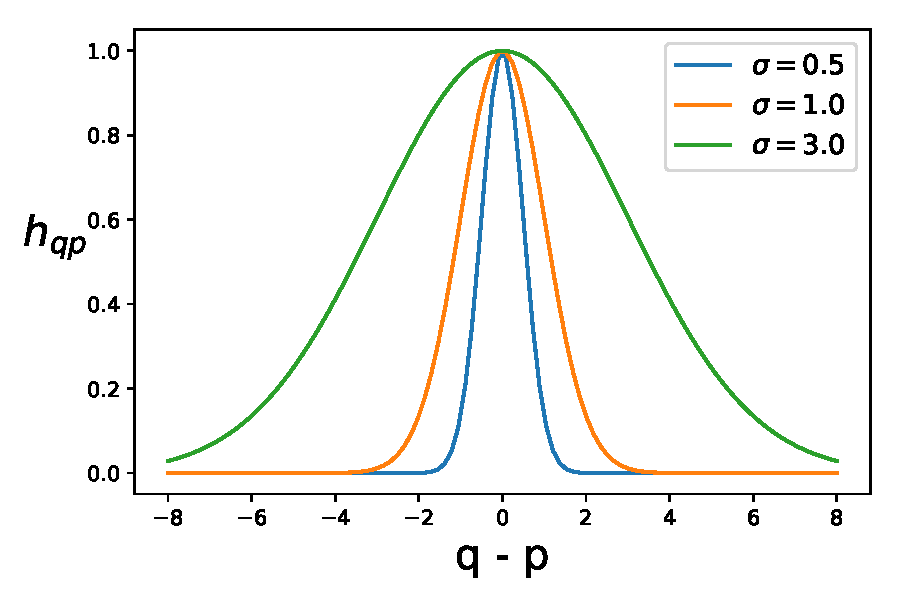
\includegraphics[width=0.9\textwidth]{img/guassian_function_1d}
	\notesonly{\captionof{figure}{In the case of a 1D map}}
\end{center}
\end{minipage}
\begin{minipage}{0.4\textwidth}
\begin{center}
	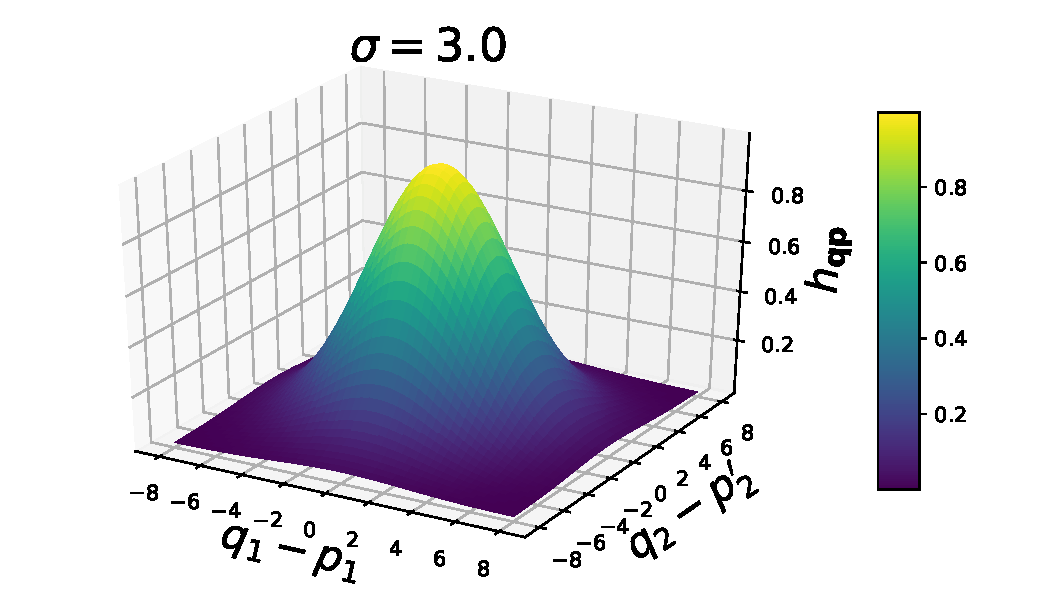
\includegraphics[width=0.9\textwidth]{img/guassian_function_2d_3Dview}
	\notesonly{\captionof{figure}{In the case of a 2D map}}
\end{center}
\end{minipage}
	\notesonly{\captionof{figure}{The Gaussian function around the winning neuron.}}
\end{center}

\end{frame}

\begin{frame}[t] \frametitle{\subsecname~$h_{\vec{q} \, \vec{p}}$} 

\svspace{-5mm}

\begin{center}
	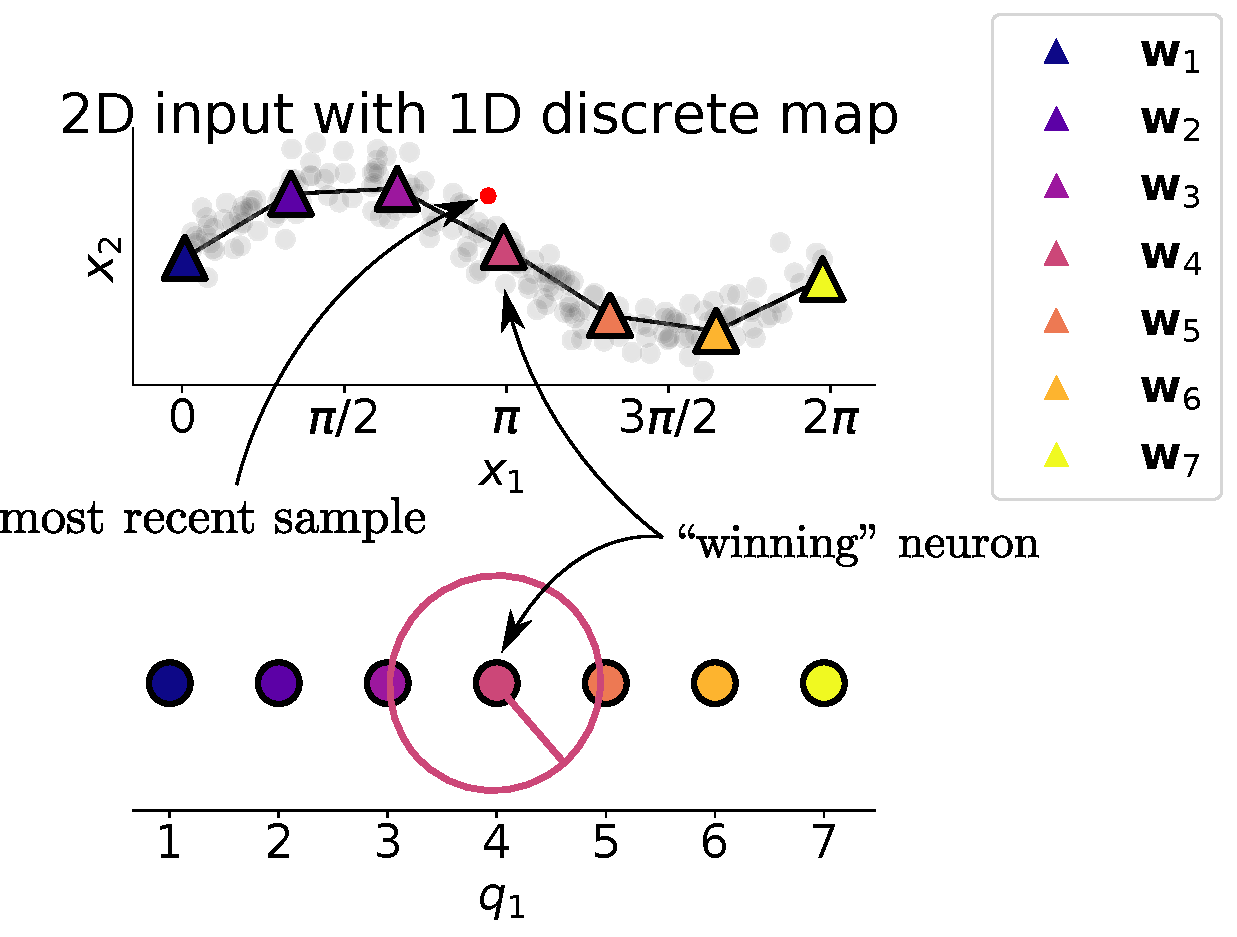
\includegraphics[width=0.44\textwidth]{img/sin_manifold_map_rbf}
	\notesonly{\captionof{figure}{The role of the neighborhood function}}
\end{center}


\svspace{-3mm}


\slidesonly{
\begin{equation}
	\Delta \vec{w}_{\vec q} = \varepsilon \cdot h_{\vec{q} \, \vec{p}} \cdot
  \big( \vec{x}^{(\alpha)} - \vec{w}_{\vec q} \big) \text{\hspace{1cm} for \textcolor{red}{all} q}
  \end{equation}
}

\svspace{-3mm}

\question{What is the effect of the width $\sigma$?}

\begin{itemize}
    \item<only@2,3> large $\sigma$ (very wide width): \only<3>{all neurons will move towards the new point.}
    \item<only@4,5> $\sigma \rightarrow 0$: \only<5>{standard on-line K-means (only update $\vec{q}=\vec{p}$)}
\end{itemize}

\end{frame}


% --------------------------------------------------------------------------
% --------------------------------------------------------------------------
\begin{frame}[t] \frametitle{\subsecname~$h_{\vec{q} \, \vec{p}}$} 
\slidesonly{
$$		h_{\vec{q} \, \vec{p}} = \exp \bigg\{ - \frac{ (\vec{q}
			- \vec{p} )^2 }{2 \sigma^2} \bigg\}
$$
}
\emph{$\sigma$ annealing}
\begin{itemize}
      \itr start with large
        $\sigma$  ($\leadsto$ neighborhood function convex over
        its support)
      \itr decrease linearly or exponentially (but
        ``slowly'') during learning.
       \itr solution depends on 
        final value of $\sigma$
        \vspace{0.5cm}
       \itr $\sigma \rightarrow 0$: minimum of the K-means clustering cost function but 
            \emph{``neighborhood preserving''}  \itr $\sigma$ small : better representation capabilities at the expense of a non-optimal clustering cost 
\end{itemize}

\question{What happens when we rush the annealing process?}

\end{frame}

\begin{frame}{The effect of rushing the annealing process}


- We ``leave the neighborhood behind''. It ``kicks into K-means mode'' too early.

\begin{minipage}{0.45\textwidth}
\begin{center}
	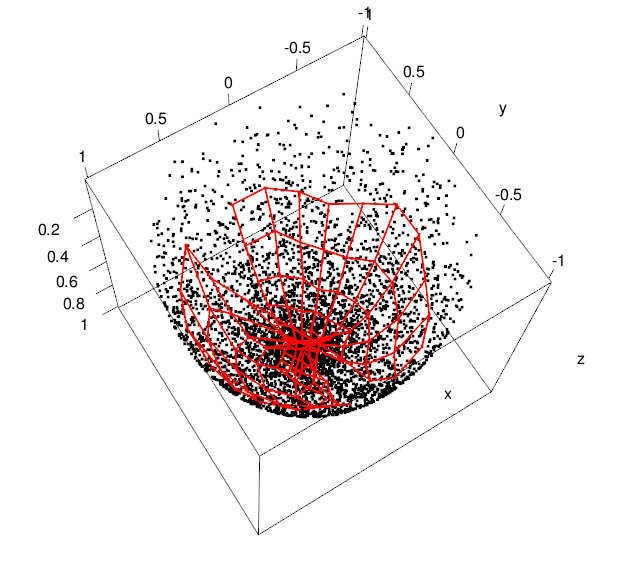
\includegraphics[width=0.9\textwidth]{img/3-bowlS2-2}
	\notesonly{\captionof{figure}{Slow annealing process preserves the neighborhood among the neurons}}
\end{center}
\end{minipage}
\begin{minipage}{0.45\textwidth}
\begin{center}
	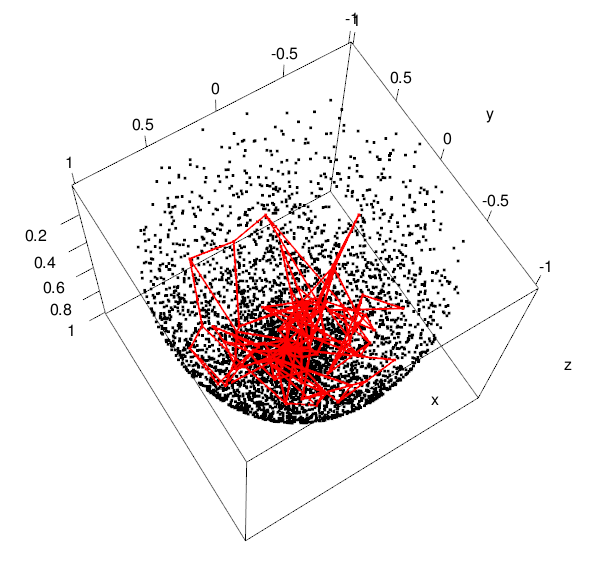
\includegraphics[width=0.9\textwidth]{img/3-bowlS2-1}
	\notesonly{\captionof{figure}{Annealing too fast ``leaves the neighborhood behind''}}
\end{center}
\end{minipage}

\end{frame}


\mode*

\clearpage

%\section{References}
%\begin{frame}[allowframebreaks] \frametitle{References}
	%\scriptsize
	%\bibliographystyle{plainnat}
	%\bibliography{bibliography}
%\end{frame}

\end{rightcolumn}
\end{paracol}

\end{document}
